 \chapter{DNA transient binding on a gold nanorod}
\label{chapter:transient}
\graphicspath{{./chapters/c5_transient_binding/figures/}}

%============================== MAIN =======================================
\begin{abstract}
  Fluorescence enhancement by plasmonic nanostructures enables the detection of dyes with low quantum yield and improves the yield of quantum solid-state light sources.
  Here we demonstrate a DNA-based transient binding method to repeatedly and reproducibly study many single molecules by fluorescence enhancement on a single nanorod at the same spot on its tip.
  Heterogeneity of excitation and emission enhancements is avoided by looking at the same nanorod and the same binding site repeatedly.
  Bleaching of the plasmonic enhanced single molecules is no longer a problem as the bleached molecules are replaced by new ones.
  We characterize the distribution of enhancement factors and binding times. We investigate the fluctuations of the enhanced signal and the long-term stability of the binding sites.
\end{abstract}

\newpage
\section{Introduction}
Plasmonic nano-structures confine light to much smaller spatial dimensions than the optical diffraction limit. They enable detection of single molecules even at micromolar or millimolar concentrations, which is otherwise extremely challenging in conventional microscopy.\cite{levene2003zeromode,punj2013a,schuller2010plasmonics}
Optical nano-antennas strongly interact with quantum emitters, modifying their excitation and emission rates, and opening new non-radiative dissipation channels.
For emitters placed at the right position, plasmonic antennas can enhance their fluorescence by two to four orders of magnitude, enabling the detection of dyes with poor quantum yields.\cite{lakowicz2005radiative,anger2006enhancement,kinkhabwala2009large,acuna2012fluorescence,yuan2013thousandfold,khatua2014resonant}
The high electric field near the antenna leads to excitation enhancement while the high local density of optical states enhances the emission rates of the emitters, often leading to improvement in the brightness.
For emitters placed close to the metal surface, the nano-structure acts as an energy sink, quenching the fluorescence.\cite{seelig2007nanoparticleinduced,muskens2007strong,acuna2012distance,matsuzaki2017strong}
However, emission enhancement and quenching are highly dependent on the position of the dye with respect to the plasmonic structures. Therefore, fluorescence enhancement in the vicinity of nanoantennas is strongly inhomogeneous, because of the inhomogeneous electric field near the plasmonic structures, and because the position of the emitters cannot be controlled accurately. 


Different approaches to study single molecules by fluorescence enhancement involve free diffusion, non-specific sticking or immobilization of the emitters around the nanostructures. All of those approaches lead to random positioning of the emitters around the antenna.\cite{pradhan2016goldnanorodenhanced,yuan2013thousandfold,zhang2017gold}
This results in inhomogeneous excitation and emission of the fluorophores.
Uniform excitation and a better understanding of the photophysics of the fluorescent probes are necessary to fully understand the activity of biological or chemical systems as the light itself can perturb the system under study.
For instance, recently we found that the different excitation rates in the near field of a gold nanorod led to variations in midpoint potential of a redox indicator (methylene blue). The origin of this change was not clear as we could not precisely control the position of the dye.\cite{zhang2017gold}
The diffusion or immobilization methods also pose a limit to the observation time of the single molecules.
Diffusion times in the near field are often faster (\SIrange{1}{1000}{\us}) than the biomolecular processes (\SI{>1}{\ms}) making it difficult to study the slower process.
Whereas molecules can be immobilized almost indefinitely by chemical binding, bleaching limits their observation time. With immobilization by chemical binding, the number of single molecules that can be studied is thus limited to one per nano-antenna.


Here, we propose a transient binding method, with which fresh single dye molecules can be transiently immobilized on the same plasmonic hot spots. Nucleic acids, in particular DNA, offer highly predictable base pairing and binding energy, providing a simple and elegant mechanism for transient binding. Transient binding of short DNA strands has been applied in a super-resolution imaging technique called DNA-PAINT.\cite{jungmann2010singlemolecule,lin2012submicrometre,schnitzbauer2017superresolution}
The necessary blinking required for super resolution is generated by the transient binding of the short dye-labeled DNA ('imager') to its complementary target ('docking') strands on the structure in vitro or in vivo.
The chemistry and kinetics of single-strand DNA (ssDNA) binding are well understood at single-molecule level and widely available, thanks to the rapid development of DNA-PAINT and DNA-based biosensors.\cite{sassolas2008dna,jungmann2010singlemolecule}
The binding time of the imager strand to the docking strand can be tuned by the electrolyte concentration, the number of base pairs, the temperature, while the distance of the molecule to the antenna can be controlled by the number of base pairs, with a resolution of \SI{0.33}{\nm} per base pair.
Moreover, as DNA has a persistence length of \SI{\sim50}{\nm}, it acts as a rigid tether, thereby stabilizing the distance between the molecule and the plasmonic nanostructure.\cite{manning2006the}


In the current study, we chose gold nanorods as the plasmonic nanoantenna because of their simple structure, the high tunability of their surface plasmon resonance (SPR) and the accessibility of their near field to bigger molecules such as proteins and other biomolecules.
The nanorod can enhance the optical excitation intensity by two to three orders of magnitude when irradiated with a resonant laser.
The fluorescence enhancement relies on the overlap of the spectrum of the dye with the SPR of the rod and the laser excitation.
The optimal distance for enhancement is \SIrange{3}{5}{\nm}; closer to the rod, fluorescence quenching will dominate; too far away from the rod, the excitation enhancement will fade.\cite{khatua2014resonant}
With a linker of 10 base pairs, the distance of the dye to the surface is \SIrange{3.5}{4}{\nm}, provided the dye is at the further end of the imager strand.
By adjusting the concentration ratio of docking strands to passivating ligands, we can tune the average number of docking strands per rod down to less than one per rod.
The binding of the docking strand being a random process, the probability of having the docking strand on one of the tips of the rod will scale similar to the ratio of near-field area to total rod area.
In the present work, we wish to characterize the enhancement factors, the binding times, and the flexibility of the docking strand attached to the nanorod. Moreover, we show that a single gold nanorod with the right binding site is enough to study fluorescent enhancement with a statistically significant number of single molecules.


%====================EXPERIMENTAL SECTION=======================
\section{Methods}
\paragraph*{Materials.} Ethanol (\SI{99.8}{\percent}), methanol (\SI{99.8}{\percent}), 3-Mercaptopropyl) trimethoxysilane (MPTS, \SI{95}{\percent}), cysteamine (\SI{98}{\percent}), thioglycolic acid (\SI{99}{\percent}), Potassium chloride (\ce(KCl)), 4-(2-Hydroxyethyl) piperazine-1-ethanesulfonic acid (HEPES, \SI{99.5}{\percent}), Bovine serum albumin (BSA, \SI{96}{\percent}), and Tris(2-carboxyethyl) phosphine hydrochloride (TCEP, \SI{98}{\percent}) were purchased from Sigma-Aldrich; 
Magnesium chloride (\ce{MgCl2}), Hydrogen peroxide (\ce{H2O2}, \SI{30}{\percent}), Sodium acetate (\ce{CH3COONa}, \SI{99}{\percent}), Potassium dihydrogenphosphate (\ce{KH2PO4}), disodium hydrogenphosphate (\ce{Na2HPO4}) from Merck;
Ammonium hydroxide (\ce{NH4OH}, \SI{30}{\percent}), Hydrochloric acid (\ce{HCl}, \SI{37}{\percent}) from Acros Organics;
succinimidyl 4-(p-maleimido- phenyl) butyrate (SMPB) from ThermoFisher.
Phosphate buffered saline (PBS) pH 7.4 contained \SI{137}{\mM} \ce{NaCl}, \SI{2.7}{\mM} \ce{KCl}, \SI{10}{\mM} \ce{Na2HPO4} and \SI{1.8}{\mM} \ce{KH2PO4}.
HEPES pH 7 buffer contain \SI{20}{\mM} HEPES. Acetate buffer pH 4 was prepared from \SI{164}{\mM} \ce{CH3COOH} and \SI{36}{\mM} \ce{CH3COONa}.


\paragraph*{Oligonucleotides.} The following DNA oligonucleotides were purchased from Integrated DNA Technologies:
\begin{itemize}
	\item DTPA-5'-ATA CAT CTA GAA ATT-3' (docking strand)
	\item -----3'-TAT GTA GAT C-Cy5-5' (imager strand)
\end{itemize}
Here DTPA represents a hexacyclic group with a dithiol that is used to strongly bind to gold, Cy5 denotes a red Cyanine dye, and A, T, C, G denote the DNA bases. Ten bases of docking strand are complementary to ten bases in the imager strand. The chemical structures and the binding scheme are shown in Figure S\ref{SIfig:AuNR-SS_bonding}.


\paragraph*{Silanization of glass surface.} Glass coverslips (Menzel-Glaser, \SI[product-units=repeat]{22x40}{\mm}, no. 1 thickness) were cleaned and activated for silanization before further functionalization.
The coverslips were sonicated in water (\SI{15}{\minute}) and ethanol (\SI{15}{\minute}). 
Then they were heated  at \SI{70}{\celsius} in a bath containing \ce{H2O}/\ce{NH4OH}/\ce{H2O2}(5:1:1) to remove organic impurities from the surface.
This step made the surface hydrophilic indicating the abundance of hydroxyl functionalities on the surface.
The cover slips were rinsed thoroughly in water and stored in ethanol for further use.
To activate the surface, the coverslips were flamed and treated for 30~min in a Teflon incubator with a \SI{1}{\percent} solution of (3-Mercaptopropyl)trimethoxysilane in methanol containing \SI{5}{\percent} glacial acetic acid.
Then the glass slides were rinsed and baked in an oven at \SI{65}{\celsius} for \SI{3}{\hour}.
This results in binding of the silane groups to the active hydroxyl groups and creates a thiol surface that can be used for conjugation with gold nanorods and for passivation of the substrate surface.


\paragraph*{Gold nanorod functionalization.} Gold nanorods (AuNRs) were synthesized using previously published seed-mediated growth in cetyl trimethyl ammonium bromide (CTAB). \cite{nikoobakht2003preparation}
The longitudinal surface plasmon of the AuNRs was \SI{640}{\nm} as obtained from the UV-vis spectrum, and their average dimensions were $\SI{90}{\nm}\times\SI{45}{\nm}$ as obtained from scanning electron microscopy images.
Excess of CTAB was removed by centrifugation and resuspension in milliQ water.
A thiolated coverslip was mounted in a homemade flow cell.
The AuNR solution was sonicated and immediately incubated in the flow cell for 10~min and then washed off with PBS buffer.
This resulted in around 10 isolated single gold nanorods per \SI{100}{\um\squared} area on the substrate.
A mixture of \SI{1}{\nM} thiolated docking strands and \SI{10}{\uM} methoxy-poly(ethylene glycol)-thiol (mPEG7-SH, MW 350) in pH 4 buffer was incubated overnight.
mPEG7-SH was used as the passivating ligand and allowed us to control the average number of docking strands on the nanorod.
The ratio between docking strands and passivating molecules was varied to get the desired number of docking strands at the tip of the nanorod.
The length and chemical nature of the passivating ligands were varied to test the flexibility of the docking strand.
Unless mentioned otherwise, the passivating ligand was mPEG.


\paragraph*{Surface passivation.} To prevent the unspecific sticking of imager strands to the surface, the rest of the glass surface was functionalized with bovine serum albumin (BSA).
This was achieved by incubating the coverslips with \SI{1}{mM} succinimidyl 4-(p-maleimidophenyl) butyrate (SMPB), \SI{20}{\uM} BSA and \SI{1}{mM} Tris(2-carboxyethyl)phosphine hydrochloride (TCEP) in HEPES pH 7 for \SI{1}{\hour}.
The succinimidyl group of SMPB binds to the BSA while its maleimide group binds to the thiol on the substrate. 
The unreacted chemicals were washed off with PBS pH 7 buffer.


\paragraph*{Imaging and time trace recording.} All the measurements were performed in a home-built confocal microscope that was equipped for Time Correlated Single Photon Counting (TCSPC).
Light from a pulsed picosecond diode laser (Power Technology, Little Rock, AR, USA) with a repetition rate of \SI{40}{\MHz} and a wavelength of \SI{635}{\nm} was passed through a narrow-band clean-up filter (Semrock LD01-640/8-25), then coupled into a single-mode optical fiber.
The output was collimated using a telescope system and reflected by a polychroic mirror (z488/633rpc) onto the back aperture of a high-numerical-aperture oil immersion objective (NA=1.4, Olympus UPLSApo 100x) and then focused to a diffraction-limited spot (\SI{300}{\nm}) on the surface of the coverslips.
An intensity of \SI[per-mode=repeated-symbol]{100}{\watt\per\cm\squared} was used to image the fluorescent objects on the surface.
Epi-fluorescence from the focal volume was collected through the same objective and focused on a pinhole for spatial filtering, and then passed through an emission filter (z488/635m "dual"-band emission filter, Chroma) to get rid of scattered laser light.
Finally, the fluorescence light was focused onto the active area of an avalanche photodiode (SPCM AQRH-15, Perkin Elmer Inc., USA).
The data was recorded by PicoHarp 300 (PicoQuant GmbH, Berlin, Germany) in time-tagged-time-resolved (t3r) mode which stores both arrival time and micro-time (time after laser excitation) of each photon.


Fluorescence images of the surface of the substrate were acquired by scanning a \SI[product-units=power]{10x10}{\um} area with a step size of \SI{50}{\nm} and a dwell time of \SI{1}{\ms}.
As the nanorods have very short photoluminescence lifetimes (shorter than the instrument response function IRF), they are easy to distinguish from the background of Cy-5 dye, with much longer fluorescence lifetime (see Figure S\ref{SIfig:trans_int_lt}).
The locations of the nanorods were saved and time traces were recorded for \SI{100}{\s} by parking the laser on the nanorods.
The laser intensity was \SI[per-mode=repeated-symbol]{10}{\watt\per\cm\squared}, 10 times smaller than the one used for imaging.
The nanorods with the desired number of transient-binding sites (inferred from the number of intensity levels) and fluorescence enhancement factor were selected for further measurements at different experimental conditions and durations.
%=======scheme========
\begin{figure}
	\centering
	\includegraphics[width=\linewidth]{scheme}
	\caption{\textbf{Transient binding schematic:}(left) Nanorods are immobilized on a thiolated glass surface and functionalized with docking strands and passivating ligands (mPEG7-SH).
	The coverslip surface is passivated with BSA to prevent non-specific sticking of imager strands to the glass.
	The imager-Cy5 strands in the solution  are shown with a gray dot on one end representing unenhanced fluorescence.
	One of the imager is bound to the docking strand at the tip of the nanorod and is shown with a bright red spot representing plasmon-enhanced fluorescence.
	(right) Reversible transient binding on the docking sites on a nanorod. The docking strand at the tip of the nanorod gives rise to enhancement while the one on the side of the rod exhibits no enhancement.}
  	\label{sch_trans:setup}
\end{figure}


\section{Results and discussion}
%========one vs many binding sites========
\paragraph{Number of binding sites.} The average number of docking strands on a gold nanorod is controlled simply by changing the concentration ratio between the docking DNA and mPEG7-SH.
Figure \ref{fig:timetrace1vsmany}(a) shows the time trace of transient binding on a gold nanorod with the ratio between docking and passivating strand maintained at 1:2000 and Figure \ref{fig:timetrace1vsmany}(c) at a ratio of 1:10000.
The concentration of imager strand was \SI{100}{\nM} with \SI{500}{\mM} \ce{NaCl} in PBS pH 7.4 buffer.
At ratio 1:2000, intensity bursts with different heights were observed and $5$ different peak heights can be distinguished from the intensity histogram with the maximum count rate at \SI{120}{ kcps} indicating an enhancement factor of $\sim60$ taking the count rate of un-enhanced imager as \SI{2} { kcps} (see Supporting Information, Fig S\ref{SIfig:timetrace_only_Cy5}).
The different peak heights are shown by the dashed lines and the numberings are done in increasing order of count rates.
The highest intensity shown by the arrow has two step-wise intensity changes resulting from two binding and unbinding events occurring during the same burst.
At ratio 1:10000, two intensity levels can be clearly distinguished both from the time trace and intensity histogram with the maximum enhancement factor of $\sim10$.
In all measurements, we adapted the laser power to the bursts to be detected, down to a factor of two in enhancement.
\begin{figure}[ht]
	\centering
	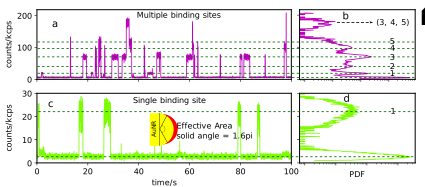
\includegraphics[width=\textwidth]{timetrace1vsmany}%width=\textwidth
	\caption{Time traces of transient binding of \SI{100}{\nM} imager with the docking sites on a gold nanorod with ratios between docking and passivating ligands of 1:2000 (a) and of 1:10000(c).
	The corresponding intensity histograms are shown on the right (b, d).
	The dashed lines connect the peaks in the histogram to the intensity levels in the time trace and the numberings are done in increasing order of the intensities.
	The arrow represents the combination of any two arbitrary levels from 1 to 5. 
	}
  	\label{fig:timetrace1vsmany}
\end{figure}


The gold nanorods were completely functionalized with mPEG7-SH and docking strands by overnight incubation.
Hinterwirth et al. showed that the coverage of \ce{PEG_7} on gold nanoparticles is \SI{4.29}{\per\nm\squared} and the packing density is mostly dependent on the steric hindrance rather than the chemical nature of the ligand.\cite{hinterwirth2013quantifying}
Therefore, a nanorod with dimensions \SI[product-units=repeat]{90x45}{\nm} should bind $5.5\times10^4$ chains, assuming similar reactivity of the passivating ligands and the docking strands.
At ratio 1:2000 between docking and mPEG7, out of ${\sim}27$ docking strands on the gold nanorod, ${\sim}5$ docking sites are observed through the fluorescence enhancement of imager strands by the gold nanorod.
Similarly, at 1:10000 ratio between docking and mPEG7 strands, ${\sim}1$ docking site is observed out of ${\sim}5$ docking strands on the nanorod.
The ratiometric study at two concentrations shows that \SI{20}{\percent} of the attached docking strands show fluorescence enhancement.
Assuming uniform distribution of the docking strands on the nanorod surface, the effective area on the nanorod for fluorescence enhancement can be calculated as \SI{20}{\percent} of its total area. We can thus estimate that the hot spots leading to a fluorescence enhancement larger than 2 times present an area of about \SI{1500}{\nm\squared} around each tip. This effective area will depend on the spectral overlap of the SPR of the rod with the dye spectra and laser, on the quantum yield of the dye, and on the distance of the dye to the surface of the rod.


One of the motivations for the present study is to observe the enhancement over and over again for the same binding site.
Figure S\ref{SIfig:bleaching_free_longtrace} shows transient binding on three different gold nanorods with different enhancement factors.
The two peaks in the intensity histogram of each rod and the absence of multi-step intensity bursts indicate that there is only one observable docking strand.
The narrow distribution of binding and unbinding times of imager strands on each particular nanorod over a time scale of \SI{1000}{\s} indicates that there is little variation in the DNA binding site over time.
However, the frequency of binding and unbinding varied from nanorod to nanorod, even for rods with a similar enhancement factor (Fig S\ref{SIfig:bleaching_free_longtrace}A, C).
This variation can be attributed to the different local environments in the PEG brush around each individual binding site, which can hinder the approach and binding of the imager strand to the docking strand.
For very long experiments (\SI{\sim1}{\hour}), we observed that the intensity bursts may completely disappear (Fig. S\ref{SIfig:dissociation_transbind}).
Deliberately applying high laser power also caused the transient binding to disappear, while some short bursts appeared.
Goodman et. al.\cite{goodman2016understanding} showed that Au-S bonds can break under some mW of pulsed laser irradiation or hundreds of mW of continuous wave (CW) laser illumination.
We attribute the short bursts appearing after irradiation with high power to non-specific sticking of imager strands to the rod. Indeed, not only the docking strands may have been released, but also some of the PEG passivating ligands, leaving comparatively free patches of bare gold surface.
While this light-induced dissociation can be useful for controlled release and delivery of drugs, it is detrimental to our transient binding experiments, where we wish to keep the docking strand permanently attached.
However, the dissociation of the docking strand from the gold can be delayed by using a CW laser instead of the pulsed laser employed in the current study.


%========Cysteamine vs peg========
\paragraph{Flexibility of the docking strand.} Different passivating ligands have been tested to understand their effect on the binding kinetics of imager and docking strands.
Two short linkers (less than \SI{1}{\nm} length), cysteamine with a basic head group (negative charge), and thioglycolic acid with a positive head group, were compared with the longer linker mPEG7-SH (\SI{\sim3.5}{\nm} length).
A transient-binding trace of a cysteamine-functionalized and of a PEG-functionalized nanorod can be seen in Figure \ref{fig:timetraceCysvsPeg}.
The intensity bursts for the cysteamine-functionalized nanorod are much noisier than the bursts of the PEG-functionalized nanorod.
We characterize the fluctuations of the fluorescence bursts by their autocorrelation function. We calculated the autocorrelation function for each of the intensity bursts. The averaged correlation functions of each time trace are shown in Figure \ref{fig:timetraceCysvsPeg}(C) for  PEG (green), cysteamine (magenta) and thioglycol (red) functionalization.
The autocorrelation of cysteamine and thioglycol-functionalization shows two exponential components while the autocorrelation for PEG shows a single exponential decay.
\begin{figure}[ht]
	\centering
	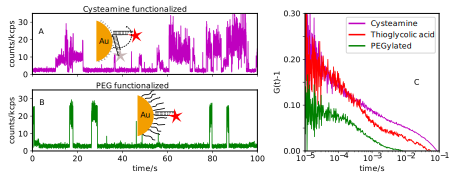
\includegraphics[width=\textwidth]{timetraceCysvsPeg}
	\caption{\textbf{Flexibility of the docking strand:} Time trace of transient binding on a gold nanorod with cysteamine (\ce{C2H7NS})(A) and mPEG7-SH (B) as passivating ligands.
	Notice the noisier intensity bursts in the case of cysteamine while the bursts for the PEGylated nanorod are much more stable.
	(C) Autocorrelation of intensity bursts for PEG (green), cysteamine (magenta) and thioglycol (red) functionalization.
	Autocorrelation values were obtained by averaging the individual autocorrelations from all bursts in each time trace. 
	Cysteamine and thioglycol have shorter chain lengths than PEG, and therefore allow more fluctuations of the distance between the nanorod and the imager dye (colored stars).}
  	\label{fig:timetraceCysvsPeg}
\end{figure}


The decay at shorter time scales (\SI{<1}{\ms}) present in all three cases is attributed to cis-trans conformational dynamics of Cy5.\cite{yeh2008tunable}
Cy5 can undergo cis-trans isomerization (Fig. S\ref{SIfig:AuNR-SS_bonding}). The trans form is planar and has stronger fluorescence, whereas the cis form has a distorted form with much lower fluorescence.
The decay at longer time scales (\SI{\sim100}{\ms}) for cysteamine and thioglycol functionalization can be attributed to the interaction of the docking strand with the functionalized nanorod surface.
Although the movement happens at nanometer scales, it can be clearly observed because of the strong dependence of the enhancement on the position with respect to the tip of the nanorod.
As the docking strand wiggles, it can come close to the surface of the nanorod resulting in quenching or it can move away from the surface of the tip resulting in enhancement.
The persistence length of DNA\cite{manning2006the} is \SI{50}{\nm}, which suggests that the movement arises from the flexibility of the tether between the docking strand and the gold surface.
However, for PEG-functionalized nanorods, the slower fluctuations are missing. We attribute this to steric hindrance by PEG chains, which prevent interactions between the hybridized DNA and the gold surface. Although the PEG brush sterically hinders the DNA motion, the imager strands can still migrate into the brush and bind to the docking strand without compromising the transient binding.


%=======countrate vs duration==========
\paragraph{Binding time.}
The binding time of the imager to the docking strand depends on many factors: the number of base pairs involved in the binding, the salt concentration, the temperature.
For the current study, the number of base pairs involved in the binding was fixed to $10$ and all the measurements were performed at \SI{500}{\mM} \ce{NaCl} and at room temperature (\SI{298}{\kelvin}).
The length of the imager strand was chosen to be $10$ base pairs to get maximum fluorescence enhancement.
Khatua et al. obtained maximum fluorescence enhancement at a distance of \SIrange{3}{5}{\nm} from the tip of the gold nanorod for the low-quantum-yield dye Crystal Violet.\cite{khatua2014resonant}
Combining the length of DNA with that of the linkers between gold and DNA and between DNA and dye, we obtain a distance of \SI{\sim4}{\nm}, which should result in an optimal enhancement.
The binding times of the imager observed from the time traces are plotted against the intensity of the bursts in the scatter plot of Figure \ref{fig:countrate_vs_duration}(A).
For low count rates we find more points with long dwell times, while at higher count rates, most of the bursts have short dwell times. 
The average burst duration clearly declines for count rates larger than \SI{\sim25}{kcps}.
We assign the reduction of burst duration for high count rates to bleaching of the dye.
For low enough count rates, the burst duration is limited by the binding time of the imager strand, rather than by the bleaching of the dye.
We thus attribute the burst duration at low count rates (below \SI{\sim25}{kcps}) to the binding time of the imager.
Above \SI{\sim25}{kcps}, the dye bleaches before the imager strand unbinds from the docking strand, resulting in a shortened burst duration.
We thus selected a maximum threshold of \SI{\sim25}{kcps} for estimating the binding kinetics.
The histogram of binding times of intensity bursts with count rate less than \SI{\sim25}{kcps} is shown in Figure \ref{fig:countrate_vs_duration}(B), which appears to decay exponentially with a characteristic time of \SI{1.13}{\s}.
The binding time of \SI{1.13}{\s} for 10-base-pair-binding at \SI{500}{\mM} \ce{NaCl} is similar to the value of \SI{5}{\s} obtained previously.\cite{jungmann2010singlemolecule}

\begin{figure}[ht]
	\centering
	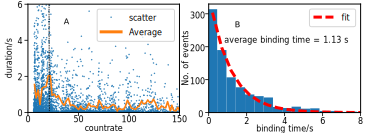
\includegraphics[width=\textwidth]{countrate_vs_duration_nophtns}
	\caption{\textbf{Binding time:} (A) Scatter plot of the burst duration versus count rate for intensity bursts in transient binding events. The data were obtained from $24$ nanorods with 1 to 5 docking sites on each of them. The vertical line indicates the count rate above which bleaching starts to govern burst duration.
	(B) Histogram of binding times of intensity bursts with count rates smaller than \SI{25}{ kcps}. The threshold was selected to exclude most bleaching events. From the exponential fit, we find an characteristic binding time of \SI{1.13}{\s}.}
  	\label{fig:countrate_vs_duration}
\end{figure}


%========Enhancement statistics=========
\paragraph{Enhancement distribution.}
Considering the strongly inhomogeneous near field of the nanoantenna, we expect a wide distribution of enhancement factors.
Figure \ref{fig:int_lt_distribution}(A) shows the distribution of burst intensities obtained for $24$ nanorods with 1 to 5 observable binding sites.
The average count rate of all those bursts was \SI{53}{kcps}, corresponding to an average fluorescence enhancement factor of $\sim25$.
The possible positions of the dye at the tip of the nanorod, assuming the tether to stand perpendicular to the surface, are shown in Figure \ref{fig:int_lt_distribution}.
The color map shows the optical intensity simulated by finite difference time domain (FDTD) in COMSOL.
The lifetime histogram of enhanced fluorescence is shown in magenta (Figure \ref{fig:int_lt_distribution}(C)) while that of unenhanced fluorescence (in absence of intensity bursts) is shown in green.
The lifetime of unenhanced Cy5 is \SI{1.8}{\ns} while the lifetime histogram of enhanced bursts cannot be distinguished from the instrument response function.
\begin{figure}[ht]
	\centering
	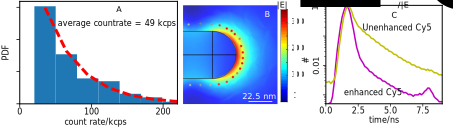
\includegraphics[width=\textwidth]{lifetime_scatplot}
	\caption{Enhancement statistics.(A) Histogram of count rates of intensity bursts of transient binding obtained from $24$ gold nanorods with 1 to 5 docking sites on each of them.
	The average count rate was \SI{53}{ kcps} with an enhancement factor of $\sim 25$.
	(B) Optical intensity map of the nanorod. The red stars indicate the positions the dye can occupy at the surface of the nanorod.
	The color bar is the normalized intensity.
	Both the enhancement factor and the number of possible binding sites are functions of the distance of the dye to the tip. The strongest enhancement corresponds to a small disk at the rod's tip, whereas the large areas on the rod sides correspond to much lower enhancements.
	(C) Lifetime histogram of all the intensity bursts found in the time trace of Figure \ref{fig:timetrace1vsmany}(a) shown in magenta. The lifetime histogram of the unenhanced fluorescence is shown in green.
	}
  	\label{fig:int_lt_distribution}
\end{figure}


As the docking strands are functionalized randomly on the nanorod without specificity to the tip, we expect to find enhancement factors corresponding to all possible positions of the dye at a fixed distance (4 nm) from the gold surface.
The maximum enhancement factor observed is 100, which is reasonable for a dye with a high quantum yield (\SI{30}{\percent}) and for an excitation enhancement of \SI{\sim300}{times} by the gold nanorod.
A previous study of the dye crystal violet showed an excitation enhancement of about hundred times. Because this dye has low quantum yield (\SI{1}{\percent}), a fluorescence enhancement of thousand-fold resulted from excitation enhancement and a 10-fold radiative enhancement. The radiative enhancement strongly depends on the quantum yield of the dye. Poorer quantum yields give rise to larger radiative enhancements. For Cy5 with a higher quantum yield, no significant radiative enhancement is expected, and the fluorescence enhancement is expected to stem mainly from excitation enhancement.
The most intense bursts come from close to the center of the tip while weak bursts originate from the sides.
The histogram of burst heights should thus be related to the distribution of light intensity at a distance of about \SI{4}{\nm} from the surface of the nanorod.


The lifetime histogram of enhanced fluorescence cannot be distinguished from the instrument response function. Therefore, the fluorescence rate (combining radiative and non-radiative rates) is enhanced by at least a factor of 10 (the lifetime of Cy5 away from the nanorod is \SI{1.8}{\ns}). However, with our current data, we cannot distinguish radiative from non-radiative contributions.
The previous study\cite{seelig2007nanoparticleinduced} shows that even at a distance of \SI{15}{\nm}, the lifetime is already reduced by a factor of 10.
As in the current study, the distance of the dye is just \SI{4}{\nm}, we expect a much shorter lifetime which requires a high-resolution TCSPC to be measurable.
% XXXrewrite this in a more neutral wayXXX As we don't expect much enhancement in the quantum yield of Cy5, quenching is probably a main contribution to the shortening of the lifetime.


\section{Conclusion}
We demonstrated the observation of many single molecules with equal enhancement factors on a single gold nanorod with a single binding site.
Different nanorods showed different enhancement factors because they presented different positions of the docking strand, in addition to different plasmon resonances.
Once a nanorod is identified with the desired enhancement factor, many single molecules can be studied with the same excitation and emission yields.
The effort to find the best enhancement factor can be reduced by specifically attaching the docking strand at the tip of the rod.
This transient binding method can be applied to different kinds of plasmonic nanostructures, where the position of the emitter can be controlled by proper DNA engineering.
Similarly, different biomolecules and quantum emitters can be studied by attaching them to the imager strand.

%=========================== SUPPORTING INFORMATION ==========================
\graphicspath{{chapters/c5_transient_binding/si-figures/}}
%============================ MAIN ==========================
\section{Supporting info}
\begin{figure}[ht]
  \centering
  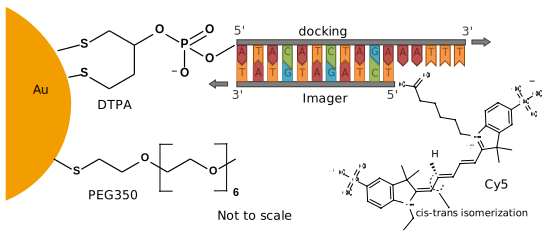
\includegraphics[width=0.8\textwidth]{AuNR-SS_bonding}
  \makeatletter
  \renewcommand{\fnum@figure}{\figurename~S\thefigure}
  \makeatother
  \caption{\textbf{Binding to gold surface} The chemical structures of different components in the transient binding scheme.
  The docking strand is attached to the nanorod through DTPA, which has two thiols attached to the gold atoms.
  The sequence of the docking and the imager strand are shown with their complementary binding.
  The imager strand is labeled with Cy5 at its 5' end.
  The rest of the nanorod surface is functionalized with PEG350, which has 9 monomers giving it a length of \SI{\sim3}{\nm}.}
  \label{SIfig:AuNR-SS_bonding}
\end{figure}

\begin{figure}[ht]
  \centering
  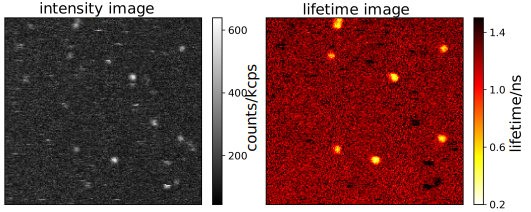
\includegraphics[width=0.8\textwidth]{trans_int_lt_img}
  \makeatletter
  \renewcommand{\fnum@figure}{\figurename~S\thefigure}
  \makeatother
  \caption{A \SI[product-units=power]{10x10}{\um} scanning image of the surface of the substrate with gold nanorod functionalized with docking strand and mPEG7-SH.
  The solution contains \SI{100}{\nM} imager strand in PBS pH 7.4 buffer with \SI{500}{\mM} \ce{NaCl}.
  The image on the left shows counts per millisecond while the image on the right shows the lifetime.
  The spots on the lifetime image correspond to the gold nanorods as they have a much shorter lifetime than the instrument response function.}
  \label{SIfig:trans_int_lt}
\end{figure}
% \subsection*{Replenish and recyacle}
\begin{figure}[ht]
  \centering
  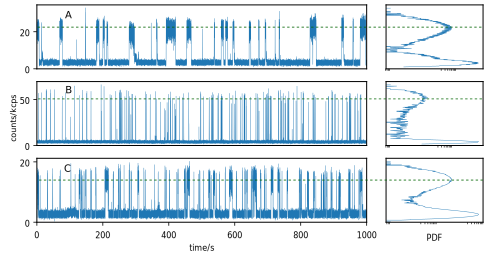
\includegraphics[width=\textwidth]{bleaching_free_longtrace}
  \makeatletter
  \renewcommand{\fnum@figure}{\figurename~S\thefigure}
  \makeatother
  \caption{\textbf{Many single molecules bind to the same binding spot on the same nanorod.} Time traces of three different nanorods, each of them with a single binding site, but with different enhancement factors.
  The histogram of intensities for each time trace is shown on the right and the two peaks indicate the presence of only one observable docking strand.
  Notice the different binding kinetics of trace A and trace C although they have similar enhancement factors.}
  \label{SIfig:bleaching_free_longtrace}
\end{figure}

\begin{figure}[ht]
  \centering
  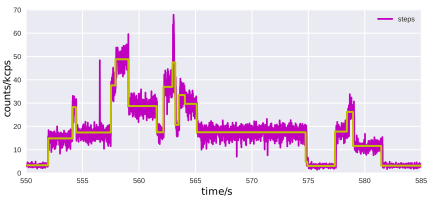
\includegraphics[width=\textwidth]{step_timetrace}
  \makeatletter
  \renewcommand{\fnum@figure}{\figurename~S\thefigure}
  \makeatother
  \caption{\textbf{Multi-step transient binding:}Time trace on a functionalized gold nanorod with multiple transient binding events appearing on top of each other.
  The association and dissociation of each imager strand can be distinguished from the step height and the time of appearance. }
  \label{SIfig: step_transbind}
\end{figure}

% \subsection*{Transient binding on substrate}
\begin{figure}[ht]
  \centering
  \includegraphics[width=\textwidth]{timetrace_only_Cy5}
  \makeatletter
  \renewcommand{\fnum@figure}{\figurename~S\thefigure}
  \makeatother
  \caption{\textbf{Transient binding without nanorod:} (A) Schematic of the transient binding.
  The docking strand was immobilized on the surface through neutravidin and biotin bonding.
  The solution contained \SI{100}{\nM} imager-Cy5 in PBS pH 7.4 buffer.
  Scanning image  in the absense (B) and presence (C) of docking strand on the surface showing the specificity of binding of the imager to the docking strand.
  (D) Time trace of transient binding on a single neutravidin-docking site at \SI{\sim 0.1}{\kW\per\cm\squared} power density, 10 times higher than the laser power used for measurement on the nanorod. The burst heights are \SI{\sim 20}{ kcps} corresponding to single imager-Cy5.
  To compare with the bursts from nanorods and calculate the enhancement factor, the count rate can be divided by 10 to match the laser power on the nanorod as the intensity varies linearly at such low powers.
  A count rate of \SI{2}{ kcps} for unenhanced Cy5 has been used in the main text. 
  }
  \label{SIfig:timetrace_only_Cy5}
\end{figure}
% \subsection*{Dissociation of docking strand}
\begin{figure}[ht]
  \centering
  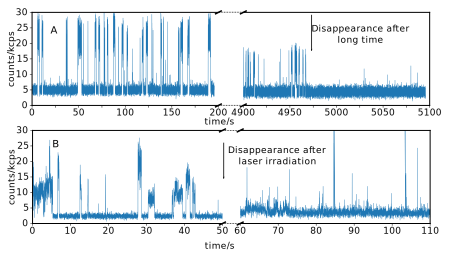
\includegraphics[width=\textwidth]{dissociation_transbind}
  \makeatletter
  \renewcommand{\fnum@figure}{\figurename~S\thefigure}
  \makeatother
  \caption{\textbf{Dissociation of docking strand.}
  (A) The time trace on the top is recorded on a gold nanorod until no docking events any more are observed.
  The transient binding events never reappeared, even after re-flushing with imager strand and realigning the laser focus.
  (B) The transient binding trace on a gold nanrod before and after irradiation with high laser power (\SI[per-mode=repeated-symbol]{1000}{\watt\per\cm\squared}, \SI{40}{\MHz}).
  }
  \label{SIfig:dissociation_transbind}
\end{figure}
% \references{chapters/c5_transient_binding/transient_binding}